\documentclass[../mciAusarbeitung.tex]{subfiles}

\usepackage[utf8]{inputenc}
\usepackage[T1]{fontenc}
\usepackage{lmodern}
\usepackage[german]{babel}
\usepackage[fixlanguage]{babelbib}
\selectbiblanguage{german}
\usepackage{amssymb}
\usepackage{graphicx}
\usepackage{url}
\usepackage{float}
\usepackage{rotating}

\title{Fachpraktikum MCI (01513) - WS 2021/22}
\author{Gruppe 2\\
	Bastian Winzen}
\date{\today}

\begin{document}
	\subsubsection{Grob - Architektur}
	Eine Gruppe von vier Entwickler:innen sollte möglichst so entwickeln können, dass sie sich nicht gegenseitig blockieren jedoch leicht Zugriff auf die Arbeit der anderen haben. Zudem sollten die einzelnen Ausarbeitungen leicht zu einem gemeinsamen Produkt verschmolzen werden können. Um diese Anforderungen bestmöglich zu erfüllen, wurde bei der Entwicklung auf die Sprache Java gesetzt. Die Arbeite wurde auf mehrere Projekte aufgeteilt. Zusammen mit dem Build und Debendency Management Tool Maven bilden sie die Basis der Entwicklung. Jedes Projekt kann für sich alleine entwickelt werden, sodass im Anschluss durch Maven die einzelnen Ergebnisse eingesammelt und in einem gemeinsamen Deployment zusammengeführt werden. Java war uns allen bekannt und zudem bieten etwaige kostenlose Java-IDEs gute Unterstützung bei der kooperativen Arbeit an Projekten.\\
	\begin{figure}[H]
	 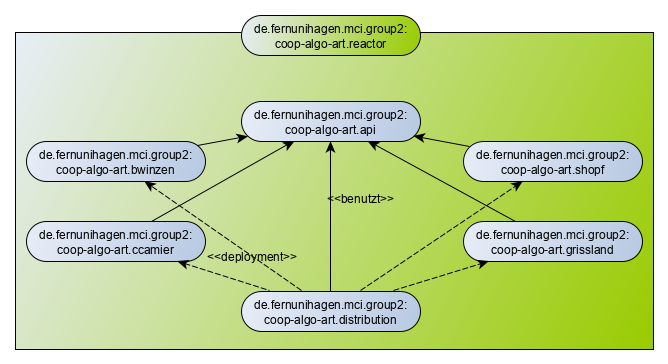
\includegraphics[width=1\linewidth]{"img/projectsDependencyTree.png"}
	 	\caption[Abhängigkeiten Projekte]{Abhängigkeiten Projekte}
	 \end{figure}
	 
	Jede:r Entwickler:in hat ein eigenes Maven/Java Projekt (de.fernunihagen.mci.group2/coop-algo-art.<Entwickler:in>) für seine Generatoren und sonstige Versuche erhalten. In den Projekten konnten alle Beteiligten nach belieben gestalten und wirken ohne die Arbeit anderer zu beeinträchtigen.\\
	Das Projekt de.fernunihagen.mci.group2/coop-algo-art.api stellt allgemeine Interfaces und Klassen zur Verfügung, wie zum Beispiel das Generatoren Interface oder den `CooperationContext'. Änderungen und Erweiterungen mussten gut abgesprochen werden, da sie Auswirkungen auf alle Entwickler:innen hatten. Jedes Projekt referenziert dieses Projekt und benutzt die enthalten Klassen oder implementiert definierte Interfaces.\\
	Am Ende sammelt das Projekt de.fernunihagen.mci.group2/coop-algo-art.distribution die anderen Projekte ein und ergänzt sie mit einem Graphical User Interface zur Konfiguration des Kunstwerkes, IO Klassen zum Speichern und Laden dieser Konfigurationen, sowie Klassen zur Präsentation und Steuerung des Kunstwerkes. \\
	Beim Bau des Distribution-Projektes werden zu den Projekten dieses Praktikums auch alle notwendigen Abhängigkeiten zu externen Bibliotheken und Frameworks zusammengetragen. Aus allen einzelnen Komponenten wird eine lauffähige jar erstellt.\\
	Der Maven Reaktor de.fernunihagen.mci.group2/coop-algo-art.reactor ummantelt die anderen Projekte. Er dient dazu Dependencies, Version und den Build-Prozess zu managen. Zu den gemanagten Abhängigkeiten zählen die `processing'-Bibliotheken, `junit' (Java-Testframework) und auch `jogl' (Java Adapter zu OpenGL). \\
	Um die Funktion als Reaktor zu erfüllen, ist jedes der für dieses Praktikum erstellten Projekte als Modul eingetragen. Jedes dieser Module hat das Reaktor Projekt als Parent gesetzt. Wird der Reaktor gebaut, so werden alle seine Module gebaut und eine lauffähige `FatJar' (Jar die alle Dependencies in sich transportiert) mit dem neusten Code-Stand kann dem Build-Verzeichnis entnommen werden.
	
	\subsubsection{Architektur - Service Sammlung}
	Aus dem beruflichen Alltag sind Fähigkeiten eines Dependency Injection Frameworks vertraut. Insbesondere das durch ein DI-Framework ermöglichte Einsammeln aller Implementierung eines Interfaces wäre für die Entwicklung der Generatoren von Vorteil gewesen.\\ 
	In OSGi(bekanntes DI-Framework) steht das sogenannte Whiteboard Pattern \cite{OsgiAlliance} dafür alle Implementierungen eines Serviceinterface an einer Stelle zu konsumieren und diese dann zentral zu benutzen oder ihre Funktionalität zur Verfügung zu stellen.\\
Auf den Einsatz eines DI-Frameworks, wie OSGi oder Springboot, im Rahmen dieses Praktikums wurde verzichtet und anstelle dessen ein Singleton benutzt, in dem Implementierungen registriert werden sollen. Dadurch wird das Debuggen vereinfachte und eine Einarbeitung in neue Technologien wird verhindert. Der Singleton `ServiceRegistry' wurde im api Projekt platziert und ist so durch jedes weitere Projekt zugreifbar. 
In den Team Meetings wurde eine Klasse `Init' definiert, die in jedem persönlichem Projekt eines Praktikumsteilnehmenden zu finden sein soll. Diese `Init' Klasse besitzt eine Methode $registerAlgorithms()$. In der `Starter' Klasse, also ganz am Beginn eines jeden Programmlaufs, werden alle `Init'-Klassen durchlaufen und die $registerAlgorithms()$-Methoden aufgerufen. \\
Jede:r Teilnehmer registriert in der eigenen Implementierung alle Services, die er/sie für das Programm bereit stellen möchte. Die Service Bereitstellung erfolgt dabei über eine Implementierung des 'ServiceFactory' Interfaces. Die Factory erzeugt beim Aufruf der entsprechenden Methode eine neue Service Instanz. Durch diese indirekte Instanziierung ist es möglich den Service zu parametrisieren, mehrere Instanzen unterschiedlicher Konfiguration gleichzeitig im System zu benutzen und trotzdem die eigentliche Implementation hinter einem Interface abstrahiert zu halten.\\
Die Implementation der `ServiceFactory' kann nicht nur durch den Aufruf der 
	\\\indent $createService(Map<String, Object> parameter)$ \\
Methode einen Service - wie zum Beispiel einen spezifischen Generator - erstellen, sondern liefert auch über die Methode \\\indent $ServiceDescription<T> getServiceDescription()$\\ ein Beschreibung von ebendiesem.\\
Die zurückgegebene `ServiceDescription' beinhaltet die ID des zugehörigen Services, einen Namen für die Anzeige auf der Oberfläche, eine Beschreibung sowie eine Definition aller spezifischen Parameter des Services.\\
Jeder der beschriebenen Parameter hat eine, im Bezug auf den aktuellen Service, eindeutige ID, einen Namen für die Anzeige, eine Beschreibung, einen Typ sowie eine typabhängige Beschreibung, die in eigene Klassen ausgelagert wurde(´xxxxRange' Klassen).\\
Im Falle einer Parameterbeschreibung eines Integer-Wertes, beinhaltet diese Beschreibung, einen minimal, maximal und einen Default-Wert. Zudem kann optional ein Inkrement festgelegt werden. Die anderen Parametertypen sind ähnlich aufgebaut.\\
	\begin{figure}[H]
	 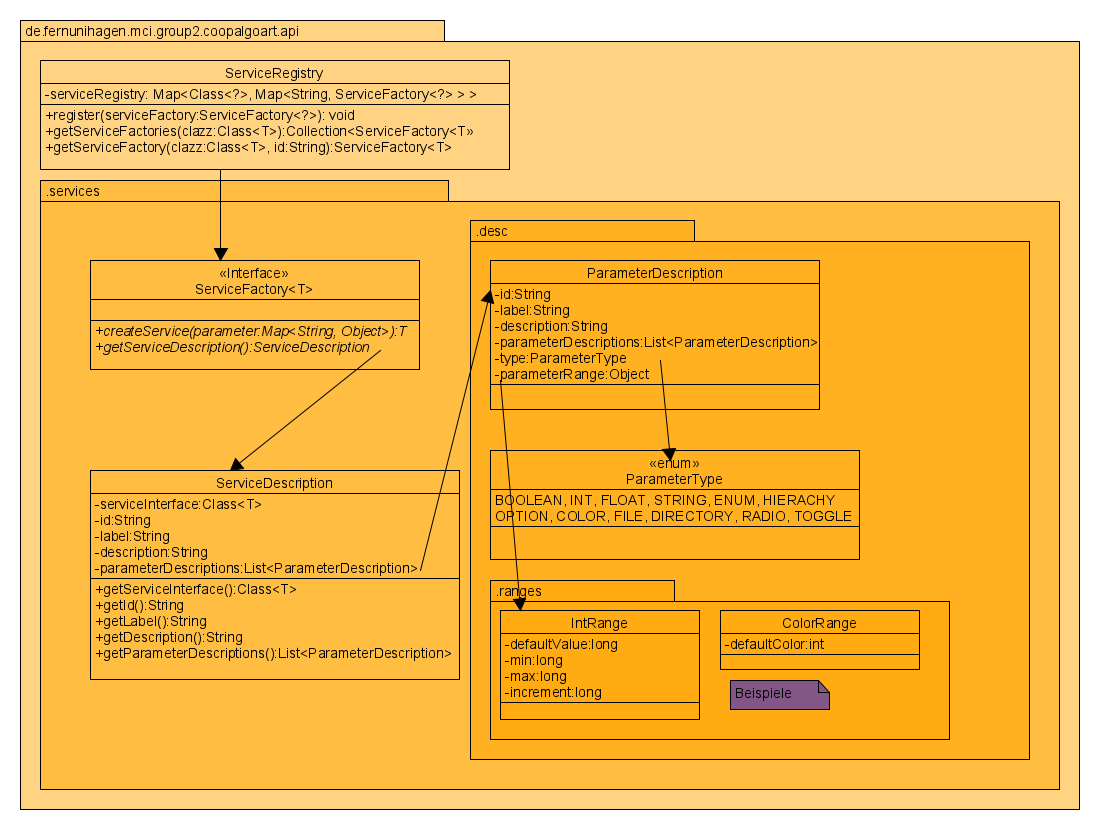
\includegraphics[width=1\linewidth]{"img/registry.png"}
	 \caption[Klassendiagramme `ServiceRegistry']{Klassendiagramme `ServiceRegistry'}
	 \end{figure}

Nachdem die `ServiceFactory's im Singleton `ServiceRegistry' registriert wurden, stehen sie im weiteren Verlauf des Programms zur Abholung bereit. Der Konsument benötigt dabei kein Wissen über die Lokalisierung der Implementierung, es bestehen keine direkten Abhängigkeiten zu den einzelnen Entwickler:innen Projekten und dennoch können Logiken aller Projekte Verwendung finden. Alles was der Anwender wissen muss, ist das gewünschte implementierte Interface und eventuell die ID des Services.\\

Das beschriebene Prinzip wird primär für die Registrierung und Bereitstellung der Generatoren genutzt, aber auch für die Registrierung unterschiedlicher Rekorder zur Aufzeichnung des Kunstwerkes. Zudem wurde angedacht die `ServiceRegistry' auch in der Kooperation zum Laden von Adapterklassen zum kooperativen Zugriff auf internen Modelle der Generatoren zu nutzen. Dies wurde im Verlaufe des Praktikums wegen seiner Komplexität verworfen.\\

Die beschriebenen `Init' Klassen können als technische Schuld gesehen werden. Durch den Aufruf dieser im `Starter' gibt es eine direkte Abhängigkeit zu den einzelnen Projekten und folglich ist das Deployment nicht dynamisch. Im Umfeld des Fachpraktikums ist der aktuelle Zustand dennoch ausreichend, da ein dynamisches Deployment nicht Teil der Aufgabenstellung ist.

\subsubsection{Architektur - Anzeige}
	Die Anzeige des Kunstobjektes ist von der Erstellung der Konfiguration unabhängig. Um Probleme mit dem Speichermanagement in dem Framework `processing' aus dem Weg zu gehen, wurde der Start jeder Anwendung in einen eigenen Prozess ausgelagert. `processing' ist anscheinend nicht dafür ausgelegt mehrfach hintereinander Fenster zu öffnen. Je nach Renderer werden einige Ressourcen nicht richtig abgebaut bzw. doppelt genutzt, wodurch immer wieder ungewollte Exceptions und Fehler aufgetreten sind.\\
	Die `Artgallery' dient der Anzeige als Startpunkt für die Visualisierung eines Kunstwerkes. Sie baut alle notwendigen Objekte für die Anzeige der Generatoren auf und verknüpft diese zu einem Ganzen. Die Klasse `Artgallery' hat eine statische `\textit{main}' Funktion (s. Abb. \ref{sequence_dia} (1)). Diese Funktion erwartet als Parameter einen Pfad zu einer Konfigurationsdatei. Um ein Instanz der `Artgallery' zu bilden, wird zuerst die Konfigurationsdatei mit Hilfe des `ConfigurationIOHelper' geladen. Der `ConfigurationIOHelper' abstrahiert den Zugriff, sowie die Umwandlung der gespeicherten Konfiguration in das `ArtConfiguration' Objekt, das die interne Repräsentation der Konfiguration darstellt (s. Abb. \ref{sequence_dia} (2)). Konnte erfolgreich eine Instanz der `ArtConfiguration' geparst werden, kann mit ihr als Parameter eine Instanz der `Artgallery' instanziiert werden (s. Abb. \ref{sequence_dia} (3)).
	
	\begin{figure}
	\begin{sideways}
    \centering
    \label{Architektur_Anzeige_Abbildung}
    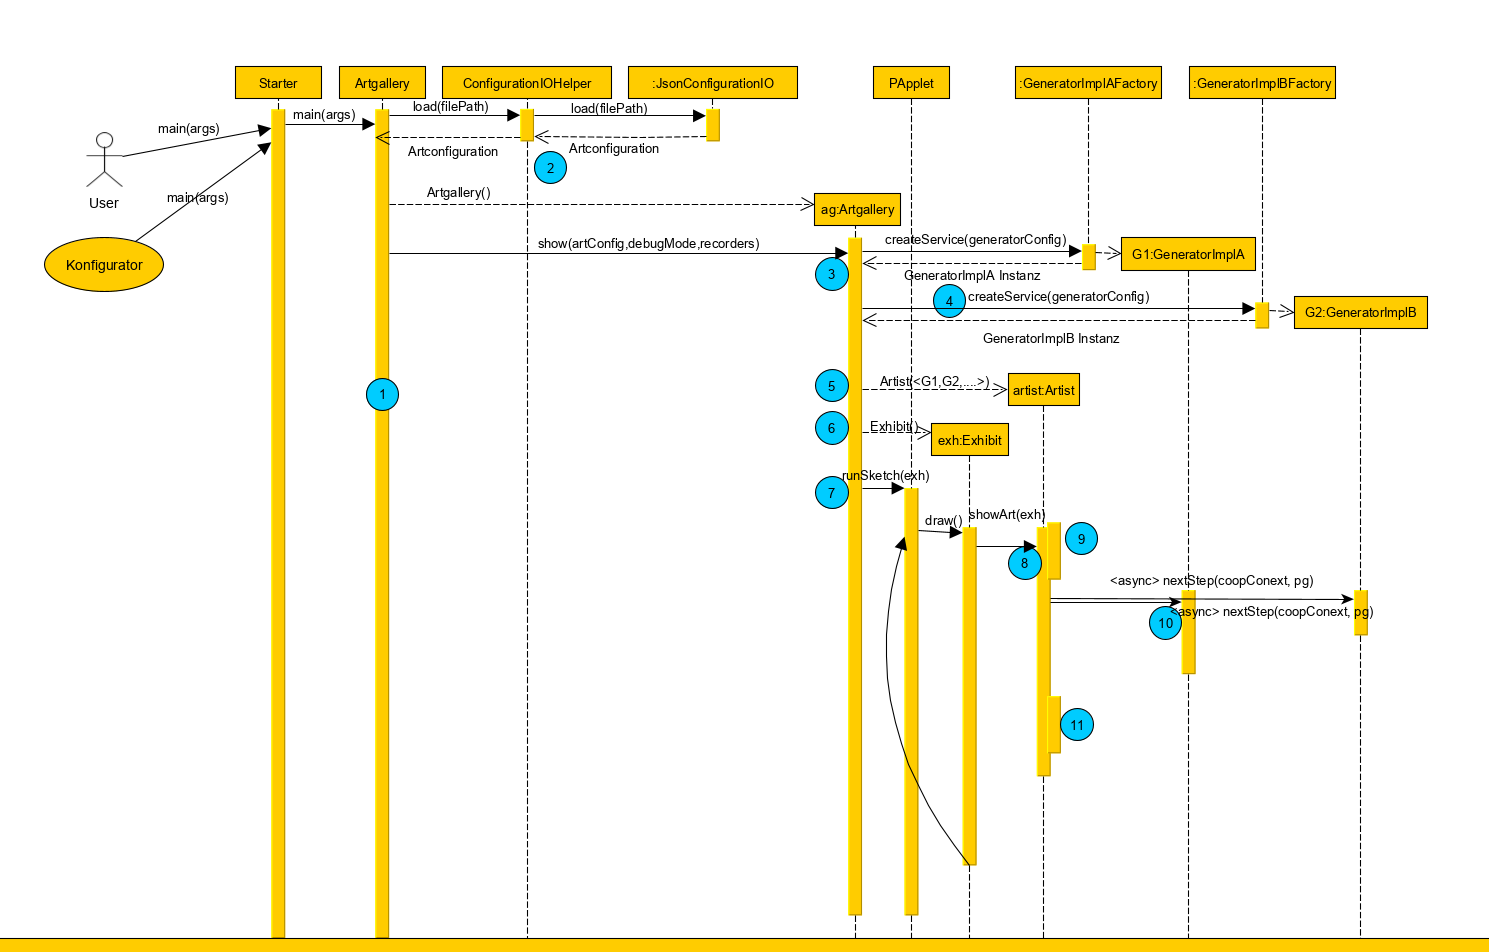
\includegraphics[width=0.95\textheight]{"img/anzeige.png"}
	\end{sideways}
	\caption[Sequenzdiagramm der Anzeige]{Sequenzdiagramm der Anzeige}
	\label{sequence_dia}
	\end{figure}
	
	Die geparste Konfiguration enthält für jeden Generator im Kunstwerk eine eigene Konfiguration. Diese enthält alle Parameter die zur Erstellung des Generators notwendig sind. Die Generatoren Konfigurationen liegen in einer Reihenfolge vor, die auch die Reihenfolge der entsprechenden Layer im ``Kunstwerk'' darstellt.
	Jede Generatoren-Konfiguration besteht aus einem allgemeinen und einem spezifischen Teil. Der allgemeine Teil beinhaltet Angaben zur Anfangsposition und zu den Dimensionen des Layers. Zudem definiert an dieser Stelle ein Parameter ob der Layer in jeder Iteration gesäubert wird oder ein Verlauf zu sehen sein soll. Zuletzt gibt eine ID Aufschluss darüber, welcher Generator erstellt werden soll.
	Der spezifische Teil der Generator-Konfiguration besteht aus Key-Value Paaren, die von der im Abschnitt `Architektur - Service Sammlung' vorgestellten `ServiceFactory' benutzt werden um eine parametrisierte Instanz des gewünschten Generators zu erstellen.\\
	Um die passende `ServiceFactory' zu finden wird  \\`\textit{\indent generatorFactory = ServiceRegistry.\\
	\indent\indent getServiceFactory(Generator.class,generatorConfig.getGeneratorId())'}\\
	aufgerufen. Ist eine `ServiceFactory' für den Zieltyp `Generator.class' unter der gesuchten ID registriert, wird diese bereitgestellt. Anschließend wird die parametrisierte Instanz des Generators mit\\ \indent `\textit{generatorFactory.createService(generatorConfig.getParameter())}' \\
	erzeugt(s. Abb. \ref{sequence_dia} (4)). \\
	Sobald alle Konfiguration in Generatoren umgewandelt wurden, wird ein `Artist' instanziiert(s. Abb. \ref{sequence_dia} (5)). Die 'Artist' dient zur Steuerung der Generatoren und der Kooperation. 
	Die `Exhibit'-Klasse ist von `PApplet' abgeleitet und dient als Schnittstelle zur `processing' Applikation. Processing ist als Standalone Applikation konzipiert wurden, um den Einstieg für Entwicklungsneulinge möglichst einfach zu halten. Dadurch ergeben sich jedoch Schwierigkeiten in der Steuerung mittels einer übergeordneten Applikation. Einige Parameter, wie z.B. die Größe des Fensters, können nur im Rahmen bestimmter Callback-Methoden an die Applikation übergeben werden.
	Die `Exhibit'-Klasse bekommt alle notwendigen Konfiguration, sowie die `Artist' Instanz im Konstruktor als Parameter übergeben(s. Abb. \ref{sequence_dia} (6)). So sind alle notwendigen Information vorhanden, wenn die `processing' Applikation über besagte Callback Methoden die Konfiguration der Applikation entgegennehmen möchte.
	 Nachdem nun alle erforderlichen Objekte erstellt wurden, wird die `processing' Applikation gestartet(s. Abb. \ref{sequence_dia} (7)).\\
	Die Implementation der Methode `\textit{showArt(Exhibit exhibit)}' des `Artist's wird in jedem Zeichenschritt des `PApplet's aufgerufen(8). Durch diesen Callback kann die Steuerung der Anzeige an den Artist ausgelagert werden. Das `Exhibit' Objekt dient nur noch als Taktgeber und Interaktionsmedium.\\
	In der aktuellen eingesetzten Implementierung der Methode `\textit{showArt(Exhibit exhibit)}' erfolgt die Abarbeitung jedes Iterationsschrittes in mehren Abschnitten.\\
	Zuerst wird der `CooperationsContext' für jeden Generator für die aktuelle Iteration berechnet(s. Abb. \ref{sequence_dia} (9)). Anschließend werden die `Generator'en aufgerufen(s. Abb. \ref{sequence_dia} (10)). Sie bekommen den errechneten `CooperationsContext' und eine eigene Zeichenfläche `PGraphics' übergeben. Die Zeichenfläche ist nach der Generatoren Konfiguration dimensioniert und wird je nach Einstellung des Verlaufs in jedem Schritt neu erstellt oder wiederverwendet. Die Generatoren können, sofern kein OpenGL-Renderer konfiguriert wurde, diesen Schritt parallel tätigen. Gerade bei lang laufenden Generatoren Implementationen ist die Parallelisierung sehr hilfreich um die User-Experience zu verbessern.\\
	Im letzten Schritt werden die Zeichenflächen zu einem Bild aggregiert und dieses auf den Bildschirm gezeichnet(s. Abb. \ref{sequence_dia} (11)). Jede Zeichenfläche wird durch den Positionsparameter im allgemeinen Bereich der zugehörigen Generatoren-Konfiguration auf der Zielzeichenfläche positioniert. Die Aggregation findet auf einem `PGraphics' Objekt mit den gewählten Maßen des Gesamtkunstwerkes statt.\\
	Schlussendlich wird das erzeugte Bild an die GUI übergeben. Durch das Zwischenzeichnen werden die Zugriffe auf die GUI minimiert und ungewollte Verzögerungen und Artefakte in der Darstellung verhindert.
 

	\subsubsection{Architektur - Konfigurator}
Das Konfigurator UI nutzt die im Kapitel `Architektur - Service Sammlung' beschrieben `ServiceDescription' um dynamisch GUI Elemente zur Konfiguration der Generatoren aufzubauen. Parametertyp und das beschreibende Range Objekt bestimmen dabei das verwendete GUI Element. \\
Grundsätzlich werden alle GUI Controls in einem 2-Spalten-Grid positioniert. Das, in der `ParameterDesciption' enthaltene, `label'-Feld wird in der linken Spalte des Grids platziert, das spezifische GUI Element in der rechten. Werden Einstellungen am Parameter vorgenommen, so wird der neue Wert unter der ID der `ParameterDesciption' in der zugehörigen Generator Konfiguration als Key-Value Paar eingetragen. Wird keine Einstellung vom User vorgenommen so findet in den meisten Fällen ein im Range Objekt enthaltener Default-Wert Anwendung.\\
Die Umwandlung von `ParameterDescription' zum GUI Control findet zentral in der `ParameterInputFactory'  statt.\\
Ein Beispiel für eine solche Umwandlung soll nun der Parameter `Anzahl' sein. Er erwartet ein Integer-Wert und soll Werte zwischen 1 und 100 enthalten. Der Default-Wert ist 1. Der in der ParameterDescription enthaltene Type Integer führt zum Aufruf der \\
`\textit{Node createIntParameter(Options generatorOptions,\\
\indent String parameterIdPrefix, ParameterDescription description, Number value)}' Methode. Dort werden die genannten Randbedingungen aus der `IntRange'-Instanz (`\textit{description.parameterRange}') gelesen und ein JavaFX Slider mit den entsprechenden Eigenschaften aufgebaut.
	

%\bibliographystyle{babplain}
%\bibliography{../mciLiteratur}
\end{document}